% Remigiusz
\section{Wielomian Jonesa}

Przed wprowadzeniem kolejnego wielomianowego niezmiennika przyjrzymy się ich historii.
Znamy już wielomian J. Alexandera, który został odkryty około roku 1928.
W 1969 J. Conway znalazł sposób na wyznaczenie wielomianu Alexandera dla dowolnego splotu przy użyciu tak zwanej relacji kłębiastej\footnote{skein relation}.
Jest to równanie wiążące wielomian splotu z wielomianami splotów o zmienionym jednym skrzyżowaniu w diagramie splotu wyjściowego.
Relacja kłębiasta okazała się kluczem do sukcesu.

Vaughan Jones, matematyk nowozelandzki, odkrył w 1984 nowy wielomian dla splotów jako produkt uboczny podczas pracy nad algebrami operatorowymi.
Odkrycie Jonesa było przełomowe, a już cztery miesiące później ogłoszono znalezienie nowego niezmiennika: wielomianu HOMFLY, którego nazwa pochodzi od pierwszych liter nazwisk odkrywców, to jest: Hoste, Ocneanu, Millett, Freyd, Lickorish, Yetter.

Aby lepiej zrozumieć wielomian Jonesa przyjrzymy się najpierw prostszej konstrukcji, nawiasowi Kauffmana.
Później zajmiemy się węzłami alternującymi.
% W tej sekcji zbadamy inny wielomianowy niezmiennik węzłów, wielomian Jonesa.
% Został odkryty w 1984 roku przez Vaughana Jonesa, znajduje zastosowanie między innymi przy badaniu węzłów przemiennych.

\subsection{Nawias Kauffmana}
Zaczniemy od zdefiniowania nawiasu Kauffmana.
Przypomnijmy, wielomian Laurenta zmiennej $X$ to formalny symbol $f=a_r X^r + \ldots + a_s X^s$, gdzie $r, s, a_r, \ldots, a_s$ są całkowite i $r \le s$.

Poszukujemy niezmiennika dla splotów o kilku prostych własnościach.
Przede wszystkim żądamy, by niewęzłowi przypisany był wielomian $1$: $\langle \NieWezel \rangle = 1$.
Po drugie chcemy móc wyznaczać nawiasy znając je dla prostszych splotów, co zapiszemy symbolicznie $\langle \PrawyKrzyz \rangle = A \langle \PrawyGladki \rangle + B \langle \LewyGladki \rangle$.
Zależy nam wreszcie na tym, by móc dodać do splotu trywialną składową: $\langle L \cup \NieWezel \rangle = C \langle L \rangle$.

Prosty rachunek pokazuje wpływ drugiego ruchu Reidemeistera na nawias:
\[
	\langle \begin{tikzpicture} [scale=0.025,baseline=-3]
			\path[TEXTARC] (0,10) .. controls (10,5) and (10,-9) .. (0,-14);
			\path[TEXTARC] (10,10) .. controls (8,9) .. (7,8);
			\path[TEXTARC] (3,4.5) .. controls (-1,0) and (-1,-4) .. (3,-8);
			\path[TEXTARC] (10,-14) .. controls (8,-13) .. (7,-12);
	\end{tikzpicture} \rangle = (A^2 + ABC + B^2) \langle \LewyGladki \rangle + BA \langle \PrawyGladki \rangle\stackrel{?}{=} \langle \PrawyGladki \rangle.
\]

Aby zachodziła ostatnia równość wystarczy (chociaż wcale nie trzeba) przyjąć $B = A^{-1}$, co wymusza na nas $C = -A^2 - A^{-2}$.
W ten sposób odkryliśmy następującą definicję.

\begin{definicja}
	\emph{Nawias Kauffmana} $\langle D \rangle$ dla diagramu splotu $D$ to wielomian Laurenta zmiennej $A$, który jest niezmienniczy ze względu na gładkie deformacje diagramu, a przy tym spełnia trzy aksjomaty:
	\begin{enumerate}
		\item $\langle \NieWezel \rangle=1$
		\item $\langle D \sqcup \NieWezel \rangle = (-A^{-2} - A^2) \langle D \rangle$
		\item $\langle \PrawyKrzyz \rangle = A \langle \PrawyGladki \rangle + A^{-1} \langle \LewyGladki  \rangle$
	\end{enumerate}
\end{definicja}

Tutaj $\NieWezel$ oznacza standardowy diagram dla niewęzła, $D \sqcup \NieWezel$ jest diagramem, który powstaje z $D$ przez dodanie nieprzecinającej go krzywej zamkniętej, zaś trzy symbole $\PrawyKrzyz$, $\PrawyGladki$ oraz $\LewyGladki $ odnoszą się do diagramów, które są identyczne wszędzie poza małym obszarem.
Diagramy $\PrawyGladki$ oraz $\LewyGladki$ nazywa się odpowiednio dodatnim (prawym) i ujemnym (lewym) wygładzeniem $\PrawyKrzyz$

\begin{lemat}
	Nawias Kauffmana dowolnego diagramu można wyznaczyć w skończonie wielu krokach.
\end{lemat}

\begin{proof}
	Jeżeli diagram $D$ ma $n$ skrzyżowań, to nieustanne stosowanie aksjomatu trzeciego pozwala na zapisanie $\langle D \rangle$ jako sumy $2^n$ składników, z których każdy jest po prostu zamkniętą krzywą i ma trywialny nawias ($\langle \MalyNieWezel \rangle = 1$).
	Nawias sumy wyznacza się korzystając z drugiego aksjomatu.
\end{proof}

Przedstawimy teraz wpływ ruchów Reidemeistera na nawias Kauffmana.

\begin{lemat}
	Pierwszy ruch Reidemeistera zmienia nawias Kauffmana zgodnie z poniższą regułą.
	Pozosałe ruchy Reidemeistera nie zmieniają nawiasu.
	\[
		% pierwszy ruch Reidemeistera
		\left\langle\begin{tikzpicture}[scale=0.05, baseline=-6]
			\clip (-12,-12) rectangle (1,7);
			\path[ARC] (-10,7) .. controls (-10,3) and (-10,0) .. (-6,-4);
			\path[ARC] (-6,0) .. controls (2,8) and (2,-10) .. (-6,-4);
			\path[ARC] (-10,-11) .. controls (-10,-8) and (-10,-5) .. (-9,-4);
		\end{tikzpicture}\right\rangle
		= -A^{-3}
		\left\langle\ \begin{tikzpicture}[scale=0.05,baseline=-6]
			\path[ARC] (-10,7) -- (-10,-11);
		\end{tikzpicture}\ \right\rangle
		\,\bullet\,
		% drugi ruch Reidemeistera
		\left\langle\begin{tikzpicture} [scale=0.04,baseline=-5]
			\path[ARC](0,10) .. controls (10,5) and (10,-9) .. (0,-14);
			\path[ARC] (10,10) .. controls (8,9) .. (7,8);
			\path[ARC] (3,4.5) .. controls (-1,0) and (-1,-4) .. (3,-8);
			\path[ARC] (10,-14) .. controls (8,-13) .. (7,-12);
		\end{tikzpicture}\right\rangle
		=
		\left\langle\ \begin{tikzpicture} [scale=0.04, baseline=-5]
		\path[ARC] (0,10) .. controls (3,8) and (3,0) .. (3,-2) .. controls (3,-4) and (3,-12) .. (0,-14);
		\path[ARC] (10,10) .. controls (7,8) and (7,0) .. (7,-2) .. controls (7,-4) and (7,-12) .. (10,-14);
		\end{tikzpicture}\ \right\rangle
		\,\bullet\,
		% trzeci ruch Reidemeistera
		\left\langle\begin{tikzpicture} [scale=0.04, auto, baseline=-6]
			\path[ARC] (-10,10) -- (-6.6,6);
			\path[ARC] (-4,3) -- (10,-14);
			\path[ARC] (10,10) -- (6.6,6);
			\path[ARC] (4,3) -- (1.6,0);
			\path[ARC] (-1.6,-4) -- (-10,-14);
			\path[ARC] (-14,-2) .. controls (-6, -2) and (-6,8) .. (0,8);
			\path[ARC] (14,-2) .. controls (6, -2) and (6,8) .. (0,8);
		\end{tikzpicture}\right\rangle
		=
		\left\langle\begin{tikzpicture} [scale=0.04, auto, baseline=-6]
			\begin{scope}[xshift=1300,rotate=180,yshift=110]
				\path[ARC] (-10,10) -- (-6.6,6);
				\path[ARC] (-4,3) -- (10,-14);
				\path[ARC] (10,10) -- (6.6,6);
				\path[ARC] (4,3) -- (1.6,0);
				\path[ARC] (-1.6,-4) -- (-10,-14);
				\path[ARC] (-14,-2) .. controls (-6, -2) and (-6,8) .. (0,8);
				\path[ARC] (14,-2) .. controls (6, -2) and (6,8) .. (0,8);
			\end{scope}
		\end{tikzpicture}\right\rangle.
	\]
\end{lemat}

\begin{proof}
Pierwszy ruch Reidemeistera:
\[
\left\langle\begin{tikzpicture}[scale=0.05, baseline=-6]
	\clip (-12,-12) rectangle (1,7);
	\path[ARC] (-10,7) .. controls (-10,3) and (-10,0) .. (-6,-4);
	\path[ARC] (-6,0) .. controls (2,8) and (2,-10) .. (-6,-4);
	\path[ARC] (-10,-11) .. controls (-10,-8) and (-10,-5) .. (-9,-4);
\end{tikzpicture}\right\rangle
\stackrel{K3}{=}
A\left\langle\begin{tikzpicture}[scale=0.05, baseline=-6]
	\clip (-12,-12) rectangle (1,7);
	\path[ARC] (-10,7) .. controls (-10,3) and (-9,-3) .. (-6,0);
	\path[ARC] (-6,0) .. controls (2,8) and (2,-10) .. (-6,-4);
	\path[ARC] (-10,-11) .. controls (-10,-8) and (-10,-1) .. (-6,-4);
\end{tikzpicture}\right\rangle
+A^{-1}\left\langle
\begin{tikzpicture}[scale=0.05, baseline=-6] 
	\clip (-12,-12) rectangle (1,7);
	\path[ARC] (-10,7) .. controls (-10,3) and (-7,-2) .. (-9,-4);
	\path[ARC] (-5,1) .. controls (2,8) and (2,-10) .. (-5,-5);
	\path[ARC] (-5,1) .. controls (-6.5,-0.5) and (-6.5,-3.5) .. (-5,-5);
	\path[ARC] (-10,-11) .. controls (-10,-8) and (-10,-5) .. (-9,-4);
\end{tikzpicture}\right\rangle
\stackrel{K2}{=}
A\left\langle\ 
\begin{tikzpicture}[scale=0.05, baseline=-6]
	\path[ARC] (-10,7) -- (-10,-11);
\end{tikzpicture}\ 
\right\rangle
+A^{-1}(-A^{-2}-A^2)\left\langle\ 
\begin{tikzpicture}[scale=0.05, baseline=-6] 
	\path[ARC] (-10,7) -- (-10,-11);
\end{tikzpicture}
\ \right\rangle
=
-A^{-3}\left\langle\ 
\begin{tikzpicture}[scale=0.05, baseline=-6] 
	\path[ARC] (-10,7) -- (-10,-11);
\end{tikzpicture}\ 
\right\rangle
\]
Pierwsza równość wynika z $K3$, druga z $K2$, trzecia jest oczywista.
Dla drugiego ruchu:
\begin{align*}
\left\langle\begin{tikzpicture} [scale=0.04,baseline=-5] 
	\path[ARC](0,10) .. controls (10,5) and (10,-9) .. (0,-14);
	\path[ARC] (10,10) .. controls (8,9) .. (7,8);
	\path[ARC] (3,4.5) .. controls (-1,0) and (-1,-4) .. (3,-8);
	\path[ARC] (10,-14) .. controls (8,-13) .. (7,-12);
\end{tikzpicture}\right\rangle
&\stackrel{K3}{=}
\phantom{-}A^{\phantom{-2}}
\left\langle\begin{tikzpicture} [scale=0.04,baseline=-5] 
	\clip (-2,-14) rectangle (12,10);
	\path[ARC] (0,10) .. controls (4.5,6) and (5.5,6) .. (10,10);
	\path[ARC] (0,-14) .. controls (4,-11) .. (6,-8) .. controls (12,0) and (-5,0) .. (3,-8);
	\path[ARC] (10,-14) .. controls (8.5,-13) .. (7,-12);
\end{tikzpicture}\right\rangle
+
\phantom{A}A^{-1}
\left\langle\begin{tikzpicture} [scale=0.04,baseline=-5]
	\clip (-2,-14) rectangle (12,10);
	\path[ARC] (10,10) .. controls (8,9) .. (7,8);
	\path[ARC] (10,-14) .. controls (8,-13) .. (7,-12);
	\path[ARC](10,10) .. controls (0,5) and (15,-4) .. (0,-14);	
	\path[ARC] (0,10) .. controls (10,5) and (-3,0) .. (3,-8);
\end{tikzpicture}\right\rangle
\stackrel{K1}{=}
-A^{-2}
\left\langle\begin{tikzpicture} [scale=0.04, baseline=-5]
	\clip (-2,-14) rectangle (12,10);
	\path[ARC] (0,10) .. controls (4.5,6) and (5.5,6) .. (10,10);
	\path[ARC] (0,-14) .. controls (4.5,-10) and (5.5,-10) .. (10,-14);
\end{tikzpicture}\right\rangle
+
\phantom{A}
A^{-1}
\left\langle\begin{tikzpicture} [scale=0.04,baseline=-5] 
	\clip (-2,-14) rectangle (12,10);
	\path[ARC] (10,10) .. controls (8,9) .. (7,8);
	\path[ARC] (10,-14) .. controls (8,-13) .. (7,-12);
	\path[ARC](10,10) .. controls (0,5) and (15,-4) .. (0,-14);	
	\path[ARC] (0,10) .. controls (10,5) and (-3,0) .. (3,-8);
\end{tikzpicture}\right\rangle
\\
&\stackrel{K3}{=}
-A^{-2}
\left\langle\begin{tikzpicture} [scale=0.04, baseline=-5]
	\clip (-2,-14) rectangle (12,10);
	\path[ARC] (0,10) .. controls (4.5,6) and (5.5,6) .. (10,10);
	\path[ARC] (0,-14) .. controls (4.5,-10) and (5.5,-10) .. (10,-14);
\end{tikzpicture}\right\rangle
+A^{-1}A
\left\langle\begin{tikzpicture} [scale=0.04, baseline=-5] 
	\clip (-2,-14) rectangle (12,10);
	\path[ARC] (0,10) .. controls (3,8) and (3,0) .. (3,-2) .. controls (3,-4) and (3,-12) .. (0,-14);
	\path[ARC] (10,10) .. controls (7,8) and (7,0) .. (7,-2) .. controls (7,-4) and (7,-12) .. (10,-14);
\end{tikzpicture}\right\rangle
+
A^{-1}A^{-1}
\left\langle\begin{tikzpicture} [scale=0.04, baseline=-5]
	\clip (-2,-14) rectangle (12,10);
	\path[ARC] (0,10) .. controls (4.5,6) and (5.5,6) .. (10,10);
	\path[ARC] (0,-14) .. controls (4.5,-10) and (5.5,-10) .. (10,-14);
\end{tikzpicture}\right\rangle
=%\phantom{-A^{-2}}
\left\langle\begin{tikzpicture} [scale=0.04, baseline=-5]
	\clip (-2,-14) rectangle (12,10);
	\path[ARC] (0,10) .. controls (3,8) and (3,0) .. (3,-2) .. controls (3,-4) and (3,-12) .. (0,-14);
	\path[ARC] (10,10) .. controls (7,8) and (7,0) .. (7,-2) .. controls (7,-4) and (7,-12) .. (10,-14);
\end{tikzpicture}\right\rangle
\end{align*}
Dla trzeciego ruchu:
\begin{align*}
\left\langle\begin{tikzpicture} [scale=0.04, auto, baseline=-6] 
	\path[ARC] (-10,10) -- (-6.6,6);
	\path[ARC] (-4,3) -- (10,-14);
	\path[ARC] (10,10) -- (6.6,6);
	\path[ARC] (4,3) -- (1.6,0);
	\path[ARC] (-1.6,-4) -- (-10,-14);
	\path[ARC] (-14,-2) .. controls (-6, -2) and (-6,8) .. (0,8);
	\path[ARC] (14,-2) .. controls (6, -2) and (6,8) .. (0,8);
\end{tikzpicture}\right\rangle
&\stackrel{K3}{=}
A
\left\langle\begin{tikzpicture} [scale=0.04, auto, baseline=-6] 
	\path[ARC] (-10,10) -- (-6.6,6);
	\path[ARC] (10,10) -- (6.6,6);
	\path[ARC] (-14,-2) .. controls (-6, -2) and (-6,8) .. (0,8);
	\path[ARC] (14,-2) .. controls (6, -2) and (6,8) .. (0,8);
	\path[ARC] (-10,-14) .. controls (0,-3) and (0,-3) .. (10,-14);
	\path[ARC] (-4,3) .. controls (0,-2) .. (4,3);
\end{tikzpicture}\right\rangle
+A^{-1}
\left\langle\begin{tikzpicture} [scale=0.04, auto, baseline=-6]
	\path[ARC] (-14,-2) -- (14,-2);
	\path[ARC] (-10,10) .. controls (-7,6) and (-4,4) .. (-4,0);
	\path[ARC] (-10,-14) .. controls (-7,-10) and (-4,-8) .. (-4,-4);
	\path[ARC] (10,10) .. controls (7,6) and (4,4) .. (4,0);
	\path[ARC] (10,-14) .. controls (7,-10) and (4,-8) .. (4,-4);
\end{tikzpicture}\right\rangle
\stackrel{R2}{=}
A
\left\langle\begin{tikzpicture} [scale=0.04, auto, baseline=-6]
	\path[ARC] (-14,-2) -- (14,-2);
	\path[ARC] (-10,-14) .. controls (0,-3) and (0,-3) .. (10,-14);
	\path[ARC] (-10,10) .. controls (0,-1) and (0,-1) .. (10,10);
\end{tikzpicture}\right\rangle
+A^{-1}
\left\langle\begin{tikzpicture} [scale=0.04, auto, baseline=-6] 
	\path[ARC] (-14,-2) -- (14,-2);
	\path[ARC] (-10,10) .. controls (-7,6) and (-4,4) .. (-4,0);
	\path[ARC] (-10,-14) .. controls (-7,-10) and (-4,-8) .. (-4,-4);
	\path[ARC] (10,10) .. controls (7,6) and (4,4) .. (4,0);
	\path[ARC] (10,-14) .. controls (7,-10) and (4,-8) .. (4,-4);
\end{tikzpicture}\right\rangle
\\
&\stackrel{R2}{=}
A
\left\langle\begin{tikzpicture} [scale=0.04, auto, baseline=-6,yscale=-1] 
	\path[ARC] (-10,10) -- (-6.6,6);
	\path[ARC] (10,10) -- (6.6,6);
	\path[ARC] (-14,-2) .. controls (-6, -2) and (-6,8) .. (0,8);
	\path[ARC] (14,-2) .. controls (6, -2) and (6,8) .. (0,8);
	\path[ARC] (-10,-14) .. controls (0,-3) and (0,-3) .. (10,-14);
	\path[ARC] (-4,3) .. controls (0,-2) .. (4,3);
\end{tikzpicture}\right\rangle
+A^{-1}
\left\langle\begin{tikzpicture} [scale=0.04, auto, baseline=-6] 
	\path[ARC] (-14,-2) -- (14,-2);
	\path[ARC] (-10,10) .. controls (-7,6) and (-4,4) .. (-4,0);
	\path[ARC] (-10,-14) .. controls (-7,-10) and (-4,-8) .. (-4,-4);
	\path[ARC] (10,10) .. controls (7,6) and (4,4) .. (4,0);
	\path[ARC] (10,-14) .. controls (7,-10) and (4,-8) .. (4,-4);
\end{tikzpicture}\right\rangle
\stackrel{K3}{=}
\left\langle\begin{tikzpicture} [scale=0.04, auto, baseline=-6] 
\begin{scope}[xshift=1300,rotate=180,yshift=110]
	\path[ARC] (-10,10) -- (-6.6,6);
	\path[ARC] (-4,3) -- (10,-14);
	\path[ARC] (10,10) -- (6.6,6);
	\path[ARC] (4,3) -- (1.6,0);
	\path[ARC] (-1.6,-4) -- (-10,-14);
	\path[ARC] (-14,-2) .. controls (-6, -2) and (-6,8) .. (0,8);
	\path[ARC] (14,-2) .. controls (6, -2) and (6,8) .. (0,8);
\end{scope}
\end{tikzpicture}\right\rangle
\end{align*}
korzystaliśmy tu z własności drugiego ruchu.
\end{proof}

Okazało się, że użycie najprostszego, I ruchu Reidemeistera, ,,psuje'' nawias!
W akcie desperacji moglibyśmy zmienić definicję, zaniechamy tego i przejdziemy do kolejnego składnika w przepisie na wielomian Jonesa.
\subsection{Spin}
Przypomnijmy, że znak skrzyżowania na diagramie to liczba $1$ lub $-1$:
$\operatorname{sign}
	\begin{tikzpicture}[scale=0.03, baseline=-3]
	\path[TEXTARC,->] (-5,-5) -- (5,5);
	\path[TEXTARC] (5,-5) -- (1.5,-1.5);
	\path[TEXTARC,<-] (-5,5) -- (-1.5,1.5);
	\end{tikzpicture}
 = +1$,
$\operatorname{sign} \begin{tikzpicture}[scale=0.03, baseline=-3]
\path[TEXTARC,->] (5,-5) -- (-5,5);
\path[TEXTARC] (-5,-5) -- (-1.5,-1.5);
\path[TEXTARC,<-] (5,5) -- (1.5,1.5);
\end{tikzpicture} = -1$.

\begin{definicja}
	Niech $D$ będzie diagramem zorientowanego splotu lub węzła.
	\textbf{Spinem} $D$ jest $w(D) = \sum_c \operatorname{sign} c$, gdzie sumowanie przebiega po wszystkich skrzyżowaniach.
\end{definicja}

\begin{przyklad}
Spinem trójlistnika w takiej wersji jest $+3$:
\[
	\begin{tikzpicture}[scale=0.035]
		\clip (-16,-16) rectangle (16,17); %nie etykietuj
		\foreach \x in {270,30, 150}
		\path[TEXTARC,->-] (15+\x:6) .. controls (130+\x:25) and (200+\x:25) .. (225+\x:10);
		\node[red] (C1) at (30:14) {\small $+1$};
		\node[red] (C2) at (150:14) {\small $+1$};
		\node[red] (C3) at (270:14) {\small $+1$};
	\end{tikzpicture}
\]
\end{przyklad}

\begin{lemat}
Tylko I ruch Reidemeistera zmienia spin:
$
w(\begin{tikzpicture}[scale=0.025, baseline=-3]
	\clip (-12,-12) rectangle (1,7);
	\path[TEXTARC] (-10,7) .. controls (-10,3) and (-10,0) .. (-6,-4);
	\path[TEXTARC] (-6,0) .. controls (2,8) and (2,-10) .. (-6,-4);
	\path[TEXTARC] (-10,-11) .. controls (-10,-8) and (-10,-5) .. (-9,-4);
\end{tikzpicture})
=
w(\ \begin{tikzpicture}[scale=0.025,baseline=-4]
	\path[TEXTARC] (-10,7) -- (-10,-11);
\end{tikzpicture}\ )-1
$, pozostałe nie mają wpływu.
Spin nie zależy od orientacji.
\end{lemat}

\begin{proof}
Proste ćwiczenie.
\end{proof}
\subsection{Wielomian Jonesa}

\begin{definicja}
\emph{Wielomian Jonesa} zorientowanego splotu to wielomian Laurenta $V(L)\in\Z[t^{1/2},t^{-1/2}]$ określony przez
\[V(L)=\left[ (-A)^{-3w(D)}\langle D\rangle\right]_{t^{1/2}=A^{-2}},\]
gdzie $D$ to dowolny diagram dla $L$.
\end{definicja}

\begin{twierdzenie}
Wielomian Jonesa jest niezmiennikiem zorientowanych splotów.
\end{twierdzenie}

\begin{proof}
%Skorzystamy z tego, że indeks zaczepienia jest niezmiennikiem.
Wystarczy pokazać niezmienniczość $(-A)^{-3w(D)}\langle D\rangle$ na ruchy Reidemeistera.
Ale
\[
(-A)^{-3
w\left(\begin{tikzpicture}[scale=0.025, baseline=-3]
	\clip (-12,-12) rectangle (1,7);
	\path[TEXTARC] (-10,7) .. controls (-10,3) and (-10,0) .. (-6,-4);
	\path[TEXTARC] (-6,0) .. controls (2,8) and (2,-10) .. (-6,-4);
	\path[TEXTARC] (-10,-11) .. controls (-10,-8) and (-10,-5) .. (-9,-4);
\end{tikzpicture}\right)}
\left\langle\begin{tikzpicture}[scale=0.025, baseline=-3]
	\clip (-12,-12) rectangle (1,7);
	\path[TEXTARC] (-10,7) .. controls (-10,3) and (-10,0) .. (-6,-4);
	\path[TEXTARC] (-6,0) .. controls (2,8) and (2,-10) .. (-6,-4);
	\path[TEXTARC] (-10,-11) .. controls (-10,-8) and (-10,-5) .. (-9,-4);
\end{tikzpicture}\right\rangle
=
(-A)^{-3
w\left(\ \begin{tikzpicture}[scale=0.025,baseline=-4]
	\path[TEXTARC] (-10,7) -- (-10,-11);
\end{tikzpicture}\ \right)+3}
(-A)^{-3}
\left\langle\ \begin{tikzpicture}[scale=0.025,baseline=-4]
	\path[TEXTARC] (-10,7) -- (-10,-11);
\end{tikzpicture}\ \right\rangle =
(-A)^{-3
w\left(\ \begin{tikzpicture}[scale=0.025,baseline=-4]
	\path[TEXTARC] (-10,7) -- (-10,-11);
\end{tikzpicture}\ \right)}
\left\langle\ \begin{tikzpicture}[scale=0.025,baseline=-4]
	\path[TEXTARC] (-10,7) -- (-10,-11);
\end{tikzpicture}\ \right\rangle.\qedhere
\]
\end{proof}

Wielomian Jonesa jest naprawdę potężnym narzędziem.
Pozwala bowiem odróżnić dowolne dwa węzły pierwsze o co najwyżej dziewięciu skrzyżowaniach.

\begin{hipoteza}
Nie istnieje nietrywialny węzeł, którego wielomian Jonesa nie odróżnia od niewęzła.
\end{hipoteza}

% \begin{twierdzenie}
% Wielomianem węzła $(m, n)$-torusowego jest
% \[
% 	\frac {t^{(m-1)(n-1):2}}{1-t^2} \cdot (1 - t^{m+1} - t^{n+1} + t^{m+n}).
% \]
% \end{twierdzenie}
\subsection{Relacja kłębiasta}
Dotychczas wyznaczyliśmy wielomian Jonesa jedynie dla trywialnych splotów.
Spowodowane jest to tym, że chociaż nawias Kauffmana jest przydatny przy dowodzeniu różnych własności, to zupełnie nie nadaje się do obliczeń.
Dużo lepszym narzędziem jest następujące twierdzenie.

\begin{twierdzenie}[relacja kłębiasta] \label{tracheotomia}
	Wielomian Jonesa spełnia równość $V(\NieWezel) = 1$ oraz relację
	\[
		t^{-1} V(L_+) - tV(L_-) + (t^{-1/2} - t^{1/2}) V(L_0) = 0,
	\]

	gdzie $L_+$, $L_-$, $L_0$ to zorientowane sploty, kóre różnią się jedynie na małym obszarze:
	$
		\begin{tikzpicture}[scale=0.03, baseline=-3]
		\path[TEXTARC,->] (-5,-5) -- (5,5);
		\path[TEXTARC] (5,-5) -- (1.5,-1.5);
		\path[TEXTARC,<-] (-5,5) -- (-1.5,1.5);
		\end{tikzpicture}
	$, 
	$
		\begin{tikzpicture}[scale=0.03, baseline=-3]
		\path[TEXTARC,->] (5,-5) -- (-5,5);
		\path[TEXTARC] (-5,-5) -- (-1.5,-1.5);
		\path[TEXTARC,<-] (5,5) -- (1.5,1.5);
		\end{tikzpicture}
	$, 
	$
		\begin{tikzpicture}[scale=0.03, baseline=-3]
		\path[TEXTARC,->] (-5,-5) .. controls (-1.5,-1.5) and (-1.5,1.5) .. (-5,5);
		\path[TEXTARC,->] (5,-5) .. controls (1.5,-1.5) and (1.5,1.5) .. (5,5);
		\end{tikzpicture}
	$.
\end{twierdzenie}

\begin{proof}
Wyraźmy wielomian Jonesa przez nawias Kauffmana i spin.
Chcemy pokazać, że
\[
A^{4}(-A)^{-3w(L_+)}\langle\PrawyKrzyz\rangle
-A^{-4}(-A)^{-3w(L_-)}\langle\LewyKrzyz\rangle
+(A^2-A^{-2})(-A)^{-3w(L_0)}\langle\PrawyGladki\rangle
=0.
\]
Ale $w(L_\pm)=w(L_0)\pm 1$, zatem to jest równoważne z $-A\langle\PrawyKrzyz\rangle +A^{-1}\langle\LewyKrzyz\rangle +(A^2-A^{-2})\langle\PrawyGladki\rangle =0$.
Z definicji nawiasu Kauffmana wnioskujemy, że
$\langle\PrawyKrzyz\rangle = A\langle\PrawyGladki\rangle+A^{-1}\langle\LewyGladki\rangle$ i $\langle\LewyKrzyz\rangle = A\langle\LewyGladki\rangle+A^{-1}\langle\PrawyGladki\rangle$.
Pierwsze równanie przemnóżmy przez $A$, drugie przez $A^{-1}$, a następnie dodajmy je do siebie.
Wtedy otrzymamy $A\langle\PrawyKrzyz\rangle-A^{-1}\langle\LewyKrzyz\rangle = A^2\langle\PrawyGladki\rangle - A^{-2}\langle\PrawyGladki\rangle$.
\end{proof}

\begin{przyklad}
	$V(
		\begin{tikzpicture}
		[scale=0.02, baseline=-3]
		\clip (-15,-9) rectangle (15,9);
		\path[TEXTARC,-<-] (1.5,-2.75) arc (-20:300:8);
		\path[TEXTARC,-<-] (-1.5,2.75) arc (160:480:8);
		\end{tikzpicture}) = -t^{5/2} - t ^{1/2}
	$ (splot Hopfa),
	$
	V(\begin{tikzpicture}[scale=0.02,baseline=-2]
	\clip (-19,-13) rectangle (19,17);
	\foreach \x in {270,30, 150}
		\path[TEXTARC,-<-] (15+\x:6) .. controls (130+\x:25) and (200+\x:25) .. (225+\x:10);
\end{tikzpicture}) = -t^4+t^3 + t
$ (trójlistnik).
\end{przyklad}
\subsection{Odwrotności, lustra i sumy}

\begin{twierdzenie}
Niech $L$ będzie zorientowanym splotem.
$V(rL)=V(L)$, $V(mL)(t)=V(L)(t^{-1})$.
\end{twierdzenie}

\begin{wniosek}
Wielomian Jonesa nie zależy od orientacji węzła (ale nie splotu!).
\end{wniosek}

\begin{proof}
Każdy węzeł ma tylko dwie orientacje, splot może mieć ich $2^n$, gdzie $n$ to liczba składowych.
\end{proof}

\begin{wniosek}
Trójlistnik nie jest równoważny ze swoim lustrem.
\end{wniosek}

\begin{proof}
W zależności od orientacji wielomianem trójlistnika jest $...$ lub $...$.
\end{proof}

\begin{twierdzenie}\label{etykieta}
Niech $L, M$ będą zorientowanymi splotami, zaś $J, K$: zorientowanymi węzłami.
\begin{enumerate}
\item $V(L \sqcup M) = (-t^{1/2} - t^{-1/2}) V(L) V(M)$,
\item $V(J \# K) = V(J) V(K)$.
\end{enumerate}
\end{twierdzenie}

\begin{proof}
Wybierzmy diagramy $D, E$ dla (odpowiednio) $L, M$.
Po podstawieniu $t^{1/2}=A^{-2}$ widzimy, że chcemy pokazać $(-A)^{-3w(D\sqcup E)}\langle D\sqcup E\rangle =(-A^2-A^{-2})(-A)^{-3(w(D)+w(E))}\langle D\rangle  \langle E\rangle$.

Oczywiście $w(D\sqcup E)=w(D)+w(E)$, więc wystarczy udowodnić, że 
\[
	\langle D\sqcup E\rangle = (-A^2-A^{-2})\langle D\rangle\langle E\rangle.
\]

Oznaczmy przez $f_1(D)$, $f_2(D)$ lewą i prawą stronę ostatniego równania.
Są to wielomiany Laurenta, które zależą tylko od $D$.
Aksjomaty Kauffmana pozwalają na pokazanie, że obie funkcje mają następujące własności:
$f_i(\NieWezel)=(-A^2-A^{-2})\langle E\rangle$, $f_i(D\sqcup\NieWezel)=(-A^2-A^{-2})f_i(D)$, $f_i(\PrawyKrzyz)=Af_i(\PrawyGladki) + A^{-1}f_i(\LewyGladki)$.
To pozwala na wyznaczenie ich wartości dla dowolnego $D$, zatem $f_1 \equiv f_2$, co kończy dowód.
\end{proof}

\begin{proof}
Narysujmy $J, K$ jako
$\begin{tikzpicture}[scale=0.02, baseline=3]
	\path[TEXTARC] (-40,0) rectangle (-20,20);
	\path[TEXTARC,-<-] (-20,17) .. controls (-5,17) and (-5,3) .. (-20,3);
	\node[darkblue] at (-30,10) {J};
	\path[TEXTARC] (35,0) rectangle (15,20);
	\path[TEXTARC,-<-] (15,17) .. controls (0,17) and (0,3) .. (15,3);
	\node[darkblue] at (25,10) {K};
\end{tikzpicture}$.
Rozpatrzmy sploty 
$\begin{tikzpicture}[scale=0.02, baseline=3]
	\path[TEXTARC] (-40,0) rectangle (-20,20);
	\node[darkblue] at (-30,10) {J};
	\path[TEXTARC] (30,0) rectangle (10,20);
	\path[TEXTARC] (10,3) -- (-3,9);
	\path[TEXTARC,->-] (-7,11) -- (-20,17);
	\path[TEXTARC] (-20,3) -- (-5,10);
	\path[TEXTARC,->-](-5,10) -- (10,17);
	\node[darkblue] at (20,10) {K};
\end{tikzpicture}
$, 
$\begin{tikzpicture}[scale=0.02, baseline=3]
	\path[TEXTARC] (-40,0) rectangle (-20,20);
	\node[darkblue] at (-30,10) {J};
	\path[TEXTARC] (30,0) rectangle (10,20);
	\path[TEXTARC] (-20,3) -- (-7,9);
	\path[TEXTARC,->-] (-3,11) -- (10,17);
	\path[TEXTARC] (10,3) -- (-5,10);
	\path[TEXTARC,->-] (-5,10) -- (-20,17);
	\node[darkblue] at (20,10) {K};
\end{tikzpicture}
$, 
$\begin{tikzpicture}[scale=0.02, baseline=3]
	\path[TEXTARC] (-40,0) rectangle (-20,20);
	\path[TEXTARC,-<-] (-20,17) .. controls (-5,17) and (-5,3) .. (-20,3);
	\node[darkblue] at (-30,10) {J};
	\path[TEXTARC] (35,0) rectangle (15,20);
	\path[TEXTARC,-<-] (15,17) .. controls (0,17) and (0,3) .. (15,3);
	\node[darkblue] at (25,10) {K};
\end{tikzpicture}$.
Relacja kłębiasta może zostać użyta do pokazania, że 
\[
t^{-1}V(J\#K)-tV(J\#K)+(t^{-1/2}-t^{1/2})V(J\sqcup K)=0.
\]
Ale $V(J\sqcup K)=(-t^{1/2}-t^{-1/2})V(J)V(K)$, co upraszcza się do $V(J\#K)=V(J)V(K)$ i kończy dowód.
\end{proof}
\subsection{Rozpiętość i wielomian Jonesa}

\begin{twierdzenie} \label{taitjones}
Niech $L$ posiada zredukowany, spójny, alternujący diagram o $n$ skrzyżowaniach.
Wtedy każdy diagram ma co najmniej $n$ skrzyżowaniach.
\end{twierdzenie}

To bardzo ważny rezultat, którego prawdziwość przypuszczał już P. G. Tait w XIX wieku.
Nikt nie był w stanie podać dowodu przed pojawieniem się wielomianu Jonesa w latach osiemdziesiątych.
Wyjaśnimy teraz użyte tu przymiotniki.

\begin{definicja}
Diagram jest alternujący, gdy podczas poruszania się wzdłuż splotu mijamy skrzyżowania na zmianę z góry oraz z dołu.
Diagram jest \emph{zredukowany}, gdy nie zawiera usuwalnych skrzyżowań.
Diagram jest \emph{spójny}, gdy nie można go podzielić na dwie niepuste części, które nie spotykają się na żadnym skrzyżowaniu.
\[\begin{tikzpicture}[scale=0.1]
	\path[ARC] (-5,-5) rectangle (5,5);
	\path[ARC] (-5,-3) -- (-12,0);
	\path[ARC] (-12,0)  -- (-19,3);
	\path[ARC] (-5,3) -- (-10,1);
	\path[ARC] (-14,-1) -- (-19,-3);
	\path[ARC,dotted] (-19,3) -- (-23.5,5);
	\path[ARC,dotted] (-19,-3) -- (-23.5,-5);
\end{tikzpicture}
\]
\end{definicja}

Przykładowo diagram $\begin{tikzpicture}
	[scale=0.02, baseline=-3]
	\path[TEXTARC] (0,0) circle (8);
	\path[TEXTARC] (20,0) circle (8);
\end{tikzpicture}$ nie jest spójny, ale $\begin{tikzpicture}
	[scale=0.02, baseline=-3]
	\path (1.5,-2.75) arc (-20:300:8) node (here) {};
	\path[TEXTARC] (here) arc (300:60:8);
	\path[TEXTARC] (-1.5,2.75) arc (160:520:8);
	\path[TEXTARC] (1.5,-2.75) arc (-20:20:8);
\end{tikzpicture}$ już tak.

W dowodzie przywołanego wyżej twierdzenia użyjemy rozpiętości wielomianu Jonesa.

\begin{definicja}
Niech $f$ będzie wielomianem Laurenta zmiennej $X$. Wtedy $M(f)$ [$m(f)$] to najwyższa [najniższa] potęga pojawiająca się w $f$. 
\emph{Rozpiętość} to $\operatorname{span} f = M(f) - m(f)$.
\end{definicja}

Zajmiemy się teraz nawiasem Kauffmana.
Znajdziemy wzór, który pozwala na wyznaczenie nawiasu dowolnego splotu o $n$ skrzyżowaniach (na diagramie) przez dodanie $2^n$ wyrazów.
Wzór ten okaże się użyteczny przy dowodzeniu późniejszych twierdzeń.

\begin{definicja}
Niech $D$ będzie diagramem splotu.
\begin{enumerate}
\item \emph{Stan} $D$ to funkcja $s$ ze zbioru skrzyżowań $D$ w $\{-1, +1\}$.
\item Dla ustalonego stanu $s$ dla $D$ przez $sD$ rozumiemy diagram powstały przez wygładzenie wszystkich skrzyżowań zgodnie z ich nowym znakiem ($\pm 1$), wtedy $|s|$ to suma wartości $s$.
\item Diagram dla $sD$ jest sumą zamkniętych krzywych, ich liczbę oznaczamy przez $|sD|$.
\end{enumerate}
\end{definicja}

\begin{twierdzenie}[o sumowaniu stanów]
Niech $D$ będzie diagramem splotu.
Wtedy
\[\langle D\rangle = \sum_s (-A^2-A^{-2})^{|sD|-1} A^{|s|},\]
gdzie sumujemy po wszystkich stanach $s$ dla $D$.
\end{twierdzenie}

\begin{proof}
Oznaczmy prawą stronę dowodzonej równości przez $[D]$.
Pokażemy, że spełnia ona $[\NieWezel]=1$, $[D\sqcup\NieWezel]=(-A^{-2}-A^2) [D]$ oraz $[\PrawyKrzyz] = A [\PrawyGladki] + A^{-1}[\LewyGladki]$.
Stąd wynika już, że $[D] = \langle D \rangle$.

Niewęzeł $\NieWezel$ ma tylko jeden stan $s$ z $|s| = 0$ i $|s\NieWezel| = 1$.

Zauważmy, że $D \sqcup \NieWezel$ i $D$ mają te same skrzyżowania, więc możemy utożsamiać stany $s$ dla $D$ ze stanami $u$ dla $D \sqcup \NieWezel$.
Wtedy $|u| = |s|$ oraz $|u(D \sqcup \NieWezel)| = |sD| + 1$.
Zatem
\[
	[D \sqcup \NieWezel] = \sum_u (-A^2-A^{-2})^{|u(D\sqcup\MalyNieWezel)|-1} A^{|u|} =\sum_s (-A^2-A^{-2})^{|sD|} A^{|s|} = (-A^2-A^{-2}) [D].
\]

Pozostała trzecia własność. Z definicji $A[\PrawyGladki]=\sum_u(-A^2-A^{-2})^{|u\MalyPrawyGladki|-1}A^{|u|+1}$, gdzie $u$ przebiega wszystkie stany $\PrawyGladki$.
Ale $\PrawyGladki$ to $\PrawyKrzyz$ ze skrzyżowaniem (powiedzmy, $c$) wygładzonym dodatnio, co daje bijekcję między stanami $u$ dla $\PrawyGladki$ i $s$ dla $\PrawyKrzyz$, dla których $s(c) = + 1$.
Wtedy $|s\PrawyKrzyz|=|u\PrawyGladki|$ i $|s|=|u|+1$ oraz
\[
A[\PrawyGladki] = \sum_u (-A^2-A^{-2})^{|u\,\MalyPrawyGladki|-1}A^{|u|+1} = \sum_{s(c)=1}(-A^2-A^{-2})^{|s\,\MalyPrawyKrzyz|-1}A^{|s|},
\]
podobne rozumowanie pokazuje, że $A^{-1}[\LewyGladki] = \sum_{s(c)=-1}(-A^2-A^{-2})^{|s\,\MalyPrawyKrzyz|-1}A^{|s|}$. 
Teraz wystarczy dodać do siebie dwa ostatnie równania. %: $A[\PrawyGladki]+A^{-1}[\LewyGladki] = \sum_s(-A^2-A^{-2})^{|s\,\MalyPrawyKrzyz|-1}A^{|s|} = [\PrawyKrzyz]$. 
\end{proof}

Zbadamy teraz dwa najprostsze stany dowolnego diagrau.

\begin{definicja}
Stan, który przypisuje znak $+1$ [$-1$] każdemu skrzyżowaniu, nazywamy $s_+$ [$s_-$].
\end{definicja}

Niech $D$ będzie alternującym, zredukowanym diagramem spójnym.
Wszystkie skrzyżowania mają ten sam znak.
Wybierzmy dla niego uszachowienie.
\[\begin{tikzpicture}[scale=0.2]
	\path[REGION] (-5,0) rectangle (5,-5);
	\path[REGION] (5,0) rectangle (15,5);
	\path[REGION] (15,0) rectangle (25,-5);
	\path[REGION] (25,0) rectangle (35,5);
	\path[REGION] (35,0) rectangle (45,-5);
	\node[above left, red] () at (5,0) {$+1$};
	\node[below left, red] () at (15,0) {$+1$};
	\node[above left, red] () at (25,0) {$+1$};
	\node[below left, red] () at (35,0) {$+1$};
	\path[ARC] (-5,0) -- (14,0);
	\path[ARC] (5,5) -- (5,1);
	\path[ARC] (5,-1) -- (5,-5);
	\path[ARC] (15,5) -- (15,-5); 
	\path[ARC] (16,0) -- (34,0);
	\path[ARC] (25,5) -- (25,1); 
	\path[ARC] (25,-1) -- (25,-5); 
	\path[ARC] (35,5) -- (35,-5); 
	\path[ARC] (36,0) -- (45,0);
\end{tikzpicture}\]
Zamieniając biały i czarny w razie potrzeby możemy założyć, że wszystkie skrzyżowania są dodatnie ($+1$).
Takie uszachowienie nazywamy \emph{standardowym}.
Porównajmy wygładzenie $s_+D$ z $s_-D$:
\[\begin{tikzpicture}[scale=0.12]
	\path[REGION] (-5,0) .. controls (6,0) and (5,0) .. (5,5)
	-- (15,5)
	 .. controls (15,0) and (15,0) .. (20,0)
	.. controls (25,0) and (25,0) .. (25,5)
	-- (35,5)
	.. controls (35,0) and (34,0) .. (45,0)
	-- (45,-5) --(35,-5)
	.. controls (35,0) and (35,0) .. (30,0)
	.. controls (25,0) and (25,0) .. (25,-5)
	-- (15,-5)
	.. controls (15,0) and (15,0) .. (10,0)
	.. controls (5,0) and (5,0) .. (5,-5)
	-- (-5,-5) -- (-5,0);
	
	\path[ARC] (35,5) .. controls (35,0) and (34,0) .. (45,0);
	\path[ARC] (-5,0) .. controls (6,0) and (5,0) .. (5,5);
	\path[ARC] (5,-5) .. controls (5,0) and (5,0) .. (10,0)
	.. controls (15,0) and (15,0) .. (15,-5);
	\path[ARC] (15,5) .. controls (15,0) and (15,0) .. (20,0)
	.. controls (25,0) and (25,0) .. (25,5);
	\path[ARC] (25,-5) .. controls (25,0) and (25,0) .. (30,0)
	.. controls (35,0) and (35,0) .. (35,-5);
	\path[ARC] (35,5) .. controls (35,0) and (34,0) .. (45,0);

	\node () at (20,2.5) {$s_+D$};
\end{tikzpicture} \quad
\begin{tikzpicture}[scale=0.12]
	\path[REGION] (-5,0) .. controls (6,0) and (5,0) .. (5,-5) -- (0,-5) -- (-5,-5) -- (-5,0);
	\path[REGION] (5,5) .. controls (5,0) and (5,0) .. (10,0)
	.. controls (15,0) and (15,0) .. (15,5) -- (5,5);
	\path[REGION] (15,-5) .. controls (15,0) and (15,0) .. (20,0)
	.. controls (25,0) and (25,0) .. (25,-5) -- (15,-5);
	\path[REGION] (25,5) .. controls (25,0) and (25,0) .. (30,0)
	.. controls (35,0) and (35,0) .. (35,5) -- (25,5);
	\path[REGION] (35,-5) .. controls (35,0) and (34,0) .. (45,0) -- (45,-5) -- (35,-5);

	\path[ARC] (-5,0) .. controls (6,0) and (5,0) .. (5,-5);
	\path[ARC] (5,5) .. controls (5,0) and (5,0) .. (10,0)
	.. controls (15,0) and (15,0) .. (15,5);
	\path[ARC] (15,-5) .. controls (15,0) and (15,0) .. (20,0)
	.. controls (25,0) and (25,0) .. (25,-5);
	\path[ARC] (25,5) .. controls (25,0) and (25,0) .. (30,0)
	.. controls (35,0) and (35,0) .. (35,5);
	\path[ARC] (35,-5) .. controls (35,0) and (34,0) .. (45,0);

	\node () at (20,2.5) {$s_-D$};
\end{tikzpicture}\]

Zamknięte krzywe tworzące $s_+D$ są brzegami białych obszarów uszachowienia, podczas gdy te tworzące $s_-D$ stanowią brzeg czarnych obszarów.
Zauważmy, że na każdym skrzyżowaniu są cztery różne czarne i białe obszary (nie mogą się spotkać w innych miejscach), gdyż diagram był zredukowany.

\begin{lemat}
Niech $D$ będzie spójnym diagramem splotu o $n$ skrzyżowaniach.
Wtedy $|s_+D|+|s_-D|\le n+2$, z równością dla zredukowanego i alternującego $D$.
\end{lemat}

\begin{proof}
Skorzystamy z indukcji względem $n$.
Łatwo widać prawdziwość lematu dla $n = 0$.
Załóżmy, że jest on prawdziwy dla wszystkich diagramów o $n - 1$ skrzyżowaniach, następnie ustalmy diagram $D$ o $n$ skrzyżowaniach.

Wybierzmy skrzyżowanie z $D$. Można je wygładzić na dwa sposoby, jeden z nich daje spójny diagram $D'$.
Bez straty ogólności przyjmijmy, że jest to dodatnie wygładzenie.
Wtedy zachodzi $|s_+D'| = |s_+D|$, ale $|s_-D'|=|s_-D|\pm 1$, ponieważ $s_-D'$ powstaje z $s_-D$ przez zastąpienie pewnej części
$\PrawyGladki$ z $\LewyGladki$.
To rozrywa jedną krzywą na dwa kawałki lub scala dwie krzywe w jedną.
Teraz $|s_+D|+|s_-D| = |s_+D'|+|s_-D'|\pm 1 \le (n-1)+2\pm 1 \le n+2$ (pierwsza nierówność wynika z założenia indukcyjnego).

Załóżmy, że $D$ jest spójny, alternujący i zredukowany.
Musimy pokazać, że ostatnie dwie nierówności tak naprawdę są równościami.
Pierwsza wynika z tego, że $D'$ jest spójny, alternujący i zredukowany.
Z drugiej strony $|s_-D'|=|s_-D|-1$, ponieważ przejście od $s_-D$ do $s_-D'$ skleja dwa czarne obszary.
To pokazuje drugą równość i kończy dowód.
\[\begin{tikzpicture}[scale=0.17]
	\path[REGION] (-5,0) rectangle (5,-5);
	\path[REGION] (5,0) rectangle (15,5);

	\path[ARC] (-5,0) -- (15,0);
	\path[ARC] (5,5) -- (5,1);  
	\path[ARC] (5,-1) -- (5,-5);
	
	\node[below] () at (5,-5) {$D$};
\end{tikzpicture}
\qquad\quad
\begin{tikzpicture}[scale=0.17]
	\path[REGION] (-5,0) .. controls (6,0) and (5,0) .. (5,-5) -- (0,-5) -- (-5,-5) -- (-5,0);
	\path[REGION] (5,5) .. controls (5,0) and (5,0) .. (10,0) -- (15,0) -- (15,5) -- (5,5);
	\path[ARC] (-5,0) .. controls (6,0) and (5,0) .. (5,-5);
	\path[ARC] (5,5) .. controls (5,0) and (5,0) .. (10,0) -- (15,0);

	\node[below] () at (5,-5) {$s_-D$};
\end{tikzpicture}
\qquad\quad
\begin{tikzpicture}[scale=0.17]
	\path[REGION] (-5,0) .. controls (6,0) and (5,0) .. (5,5)
	-- (15,5) -- (15,0)--(10,0)
	.. controls (5,0) and (5,0) .. (5,-5)
	-- (-5,-5) -- (-5,0);

	\path[ARC] (-5,0) .. controls (6,0) and (5,0) .. (5,5);
	\path[ARC] (5,-5) .. controls (5,0) and (5,0) .. (10,0) -- (15,0);

	\node[below] () at (5,-5) {$s_-D'$};
\end{tikzpicture} \qedhere\]
\end{proof}

\begin{lemat}
Niech $D$ będzie diagramem splotu o $n$ skrzyżowaniach.
Wtedy
\begin{enumerate}
\item $M \langle D \rangle \le n+2|s_+D|-2$
\item $m \langle D \rangle \ge -n-2|s_-D|+2$
\end{enumerate}
z równością, jeżeli $D$ jest alternujący, zredukowany i spójny.
\end{lemat}

\begin{proof}
Udowodnimy tylko pierwszą część, druga jest do niej podobna.
Dla stanu $s$ diagramu $D$ niech $\langle D \mid s\rangle :=(-A^{-2}-A^2)^{|sD|-1}A^{|s|}$.
Wzór sumujący stany przybiera postać $\langle D\rangle = \sum_s \langle D \mid s\rangle$.

Zauważmy, że $M\langle D|s\rangle=2|sD|+|s|-2$, a więc w szczególności $M\langle D|s_+\rangle=2|s_+D|+n-2$.
Gdyby udało się nam pokazać, że $M\langle D|s\rangle \le M\langle D|s_+\rangle$ dla wszystkich innych stanów $s$, dowód nierówności byłby zakończony.
Ale możemy znaleźć ciąg $s_+ = s_0$, $s_1$, \ldots, $s_r=s$, w którym $s_{i+1}$ powstaje z $s_i$ przez pojedynczą zmianę $+1$ na $-1$.

Teraz $|s_{i+1}|=|s_i|-2$, podczas gdy $|s_{i+1}D|=|s_iD|\pm 1$, ponieważ $s_{i+1}D$ uzyskujemy z $s_{i}D$ przez połączenie dwóch zamkniętych krzywych lub podział jednej zamkniętej krzywej na dwie części.
Zatem
\[
	M \langle D \mid s_{i+1} \rangle =
	2|s_{i+1}D|+|s_{i+1}|-2 =
	(2|s_iD| + |s_i| -2 ) + (\pm 2-2) \le
	M \langle D|s_i\rangle.
\]

Teraz widać już, że $M\langle D \mid s\rangle =M\langle D \mid s_r\rangle \le\ldots\le M\langle D \mid s_0\rangle=M\langle D \mid s_+\rangle$.

Pokażemy teraz, że jeśli $D$ jest zredukowany, alternujący i spójny, to nierówność zamienia się w równość.
Będzie to wynikało z  $M\langle D|s\rangle<M\langle D| s_+\rangle$
dla $s\neq s_+$, jeżeli tylko powołamy się na powyższy argument.
Wystarczy ograniczyć się do tych $s$, które powstają z $s_+$ przez zmianę pojedynczego stanu $+1$ na $-1$.
Ale to już jest oczywiste, gdyż $sD$ otrzymujemy przez sklejenie dwóch białych obszarów $s_+ D$.
\end{proof}

Możemy wreszcie zająć się rozpiętością wielomianu Jonesa.

\begin{twierdzenie}
Niech $L$ będzie zorientowanym splotem o spójnym diagramie $D$ z $n$ skrzyżowaniami.
Wtedy $\operatorname{span}(V(L)) \le n$, z równością dla zredukowanego i alternującego $D$.
\end{twierdzenie}

\begin{proof}
Pokażemy prawdziwość innego, równoważnego stwierdzenia: $\operatorname{span} \langle D\rangle\le 4n$ z równością dla zredukowanego i alternującego $D$.
Dwa poprzednie lematy mówią, że
\begin{align*}
\operatorname{span}\langle D\rangle & = M\langle D\rangle - m\langle D\rangle \le (2|s_+D|+n-2)+(2|s_-D|+n-2) \\
& = 2(|s_+D|+|s_- D|)+2n-4 \le 2(n+2)+2n-4 = 4n. \qedhere
\end{align*}
\end{proof}

Jesteśmy już w stanie podać dowód twierdzenia \ref{taitjones} wspomnianego na początku sekcji.

\begin{proof}
Założenia mówią nam, że $\operatorname{span} (V(L)) = n$.
Gdyby istniał diagram o mniejszej liczbie skrzyżowań, mielibyśmy $\operatorname{span} (V(L)) < n$, co prowadzi do sprzeczności.
\end{proof}

Wyznaczanie wielomianu Jonesa dla splotu jest uciążliwe, jednak czasami możemy oszacować jego rozpiętość korzystając z następujących nierówności:

\begin{wniosek}
Niech $L$ będzie zorientowanym splotem ze spójnym diagramem $D$ o $n$ skrzyżowaniach. Wtedy
\[\frac{3w(D)-2|s_+D|+2-n}{4} \le m(V(L) \textrm{ oraz } M(V(L)) \le \frac{3w(D)+2|s_-D|+n-2}{4},\]
z równością dla zredukowanego i alternującego $D$.
\end{wniosek}

\begin{proof}
Proste ćwiczenie.
\end{proof}
\subsection{Wielomian HOMFLY}
Po tym, jak Jones przedstawił światu swój wielomian w 1984 roku, matematycy zaczęli szukać jego uogólnienia zależnego nie od jednej, lecz dwóch zmiennych.
Pierwszym takim niezmiennikiem węzłów okazał się wielomian (Laurenta) HOMFLY.

\begin{definicja}
\emph{Wielomian HOMFLY} zorientowanego splotu to wielomian Laurenta zależny od $m$ i $l$, który spełnia dwa  aksjomaty: $P(\NieWezel) = 1$ oraz $l P(L_+) + l^{-1} P(L_-) + mP(L_0) = 0$ (przy oznaczeniach z twierdzenia \ref{tracheotomia}).
\end{definicja}

\begin{twierdzenie} Wielomian HOMFLY dla sum:
\begin{enumerate}
	\item $P(L_1 \sqcup L_2) = - (l + l^{-1}) m^{-1} P(L_1) P(L_2)$.
	\item $P(L_1 \# L_2) = P(L_1) P(L_2)$.
\end{enumerate}
\end{twierdzenie}

Okazuje się, że wielomian HOMFLY uogólnia jednocześnie wielomiany Jonesa i Alexandera:

\begin{twierdzenie} Dla dowolnego (splotu / węzła, nie/zorientowanego?) zachodzą równości:
\begin{itemize}
\item $V(t) = P(l = it^{-1}, m = i(t^{-1/2} - t^{1/2}))$,
\item $\Delta(t) = P(l = i, m = i(t^{1/2} - t^{-1/2}))$.
\end{itemize}
\end{twierdzenie}

Zaletą wielomianu HOMFLY jest to, że zazwyczaj wykrywa chiralność\footnote{węzeł chiralny: posiadający formy różnej handedness, które nie są lustrzanie symetryczne}, ale nie odróżnia enancjomerów węzłów 09-042, 10-048, 10-071, 10-091, 10-104, oraz 10-125.

Mutanty mają ten sam wielomian HOMFLY.
Okazuje się, że istnieje nieskończenie wiele parami różnych węzłów o tym samym wielomianie (Kanenobu 1986).
Przykłady:  (05-001, 10-132), (08-008, 10-129) (08-016, 10-156), oraz (10-025, 10-056) (Jones 1987).

M. B. Thistlethwaite wyznaczył HOMFLY dla tych, które mają mniej niż 14 skrzyżowań.
\subsection{Węzły pierwsze}

Liczby pierwsze znane z teorii liczb mają swój odpowiednik wśród węzłów.
Odpowiednik ten jest ściśle związany z operacją sumy spójnej, którą teraz zdefiniujemy.

\begin{definicja}
Niech $J$ i $K$ będą zorientowanymi węzłami.
Aby otrzymać ich sumę spójną, rozdzielamy je płaszczyzną i wybieramy gładką ścieżkę $\gamma \colon [0,1] \to \R^3$ z punktu $\gamma(0)$ w $J$ do $\gamma(1)$ w $K$, która nie przecina żadnego z diagramów.
Usuwamy krótkie łuki przy $\gamma(0)$ i $\gamma(1)$, po czym łączymy węzły ścieżką równoległą do $\gamma$.
\[
\begin{tikzpicture}[scale=0.05]
	% Figure Eight
	\path[ARC] (0,-10) .. controls (8,0) and (-8,0) .. (-8,8);
	\path[ARC] (-8,12) .. controls (-8,20) and (20,20) .. (1,1);
	\path[ARC] (5,10) .. controls (-30,16) and (-12,-22) .. (-3,-13);
	\path[ARC,decoration={markings, mark=at position .75 with {\arrow{<}}},postaction={decorate}]
		(-3,-3) .. controls (-7,-7) and (0,-15) .. (5,-15)
		.. controls (15,-15) and (19,7) .. (10,9);
	\node at (0,-20) {$J$}; 
	% Trefoil
	\path[ARC] (50+0,10) .. controls (50+10,0) and (50+-10,0) .. (50+0,-10);
	\path[ARC] (50+-1.5,1.5) .. controls (50+-6,6) and (50+-3,17) .. (50+10,12)
		.. controls (50+23,7) and (50+15,-20)  .. (50+3,-13);
	\path[ARC,decoration={markings, mark=at position .6 with {\arrow{>}}},postaction={decorate}]
		 (50+1.5,-1.5) .. controls (50+6,-6) and (50+3,-17) .. (50+-10,-12)
		.. controls (50+-23,-7) and (50+-15,20)  .. (50+-3,13);
	\node at (0,-20) {$J$};
	\node at (50,-20) {$K$};
\end{tikzpicture}
\begin{tikzpicture}[scale=0.05]
	%Figure-eight
	\path[ARC] (0,-10) .. controls (8,0) and (-8,0) .. (-8,8);
	\path[ARC]
		(-8,12) .. controls (-8,20) and (20,20) .. (1,1);
	\path[ARC] (5,10) .. controls (-30,16) and (-12,-22) .. (-3,-13);
	\path[ARC] (-3,-3) .. controls (-7,-7) and (0,-15) .. (5,-15);
	%trefoil
	\path[ARC] (50+0,10) .. controls (50+10,0) and (50+-10,0) .. (50+0,-10);
	\path[ARC] (50+-1.5,1.5) .. controls (50+-6,6) and (50+-3,17) .. (50+10,12)
		.. controls (50+23,7) and (50+15,-20)  .. (50+3,-13);
	% Bottom connector
	\path[ARC,decoration={markings, mark=at position .65 with {\arrow{>}}},postaction={decorate}]
		(50+1.5,-1.5) .. controls (50+12,-15) and (50+-14,-18) .. (50+-16,-5)--
		(15,-5) .. controls (15,-10) and (10,-15) .. (5,-15);
	% Top connector
	\path[ARC,decoration={markings, mark=at position .4 with {\arrow{>}}},postaction={decorate}]
		(10,9) .. controls (15,8) and (15,3)  .. (15,0)--
		(50+-16.5,0) .. controls (50+-16.5,10) and (50+-11,17) .. (50+-3,13);
	\node at (25,-20) {$J\#K$};
\end{tikzpicture}\]

\end{definicja}

Operacja sumy spójnej określona jest jedynie dla zorientowanych węzłów, ponieważ bez orientacji istnieje drugi, być może nierównoważny sposób na połączenie diagramów.
Nie ma ona też sensu dla splotów, nawet zorientowanych, gdyż nie istnieje dla nich kanoniczny sposób na wybór, które składowe należałoby ze sobą połączyć.

\begin{twierdzenie}
Niech $J, K$ będą zorientowanymi węzłami.
Ich suma spójna jest dobrze określona i zależy jedynie od klas równoważności, a nie samych węzłów.
\end{twierdzenie}

\begin{proof}(Szkic)
Załóżmy, że mamy dane węzły $J, K$ oraz ścieżki $\gamma$, $\delta$, których używamy do stworzenia sumy $J\# K$.
Wykonujemy następujące kroki.
\begin{enumerate}
\item Kurczymy $K$.
\item Przesuwamy $K$ wzdłuż $\gamma$ tak, by leżało blisko $\gamma(0)$.
\item Przesuwamy $K$ wzdłuż $J$ od $\gamma(0)$ do $\delta(0)$.
\item Odwracamy dwa pierwsze kroki z $\delta$ w miejscu $\gamma$.\qedhere
\end{enumerate}
\end{proof}



\begin{twierdzenie}
Suma spójna jest działaniem łącznym i przemiennym.
Niewęzeł $\NieWezel$ jest jego elementem neutralnym.
\end{twierdzenie}

\begin{proof}
Przedstawmy węzły $I, J, K$ w następujący sposób:
\[\begin{tikzpicture}[scale=0.08]
%	\clip (-21,-16) rectangle (21,16);
	\path[ARC] (-50,0) rectangle (-40,-10);
	\path[ARC,-<-] (-40,-2) .. controls (-35,-2) and (-35,-8) .. (-40,-8);
	\node () at (-45,-5) {$I$};

	\path[TEXTARC, blue,->-] (-35,-5) -- node[auto] () {$\gamma$} (-25,-5);

	\path[ARC] (-20,0) rectangle (-10,-10);
	\path[ARC,->-] (-20,-2) .. controls (-25,-2) and (-25,-8) .. (-20,-8);
	\path[ARC,-<-] (-10,-2) .. controls (-5,-2) and (-5,-8) .. (-10,-8);
	\node () at (-15,-5) {$J$};
	
	\path[TEXTARC, blue,->-] (-5,-5) -- node[auto] () {$\delta$} (5,-5);
	
	\path[ARC] (10,0) rectangle (20,-10);
	\path[ARC,->-] (10,-2) .. controls (5,-2) and (5,-8) .. (10,-8);
	\node () at (15,-5) {$K$};
\end{tikzpicture}\]
Tworzymy sumy $I\#(-)$ przy użyciu $\gamma$, $(-)\#K$ przy użyciu $\delta$.
Wtedy $(I\#J)\#K$ oraz $I\#(J\#K)$ są dane przez
\[\begin{tikzpicture}[scale=0.08]
%	\clip (-21,-16) rectangle (21,16);
	\path[ARC] (-50,0) rectangle (-40,-10);
	\node () at (-45,-5) {$I$};
	\path[ARC] (-20,0) rectangle (-10,-10);
	\node () at (-15,-5) {$J$};
	\path[ARC] (10,0) rectangle (20,-10);
	\node () at (15,-5) {$K$};

	\path[ARC,-<-] (-40,-2) -- (-20,-2);
	\path[ARC,->-] (-40,-8) -- (-20,-8);

	\path[ARC,-<-] (-10,-2) -- (10,-2);
	\path[ARC,->-] (-10,-8) -- (10,-8);
\end{tikzpicture},\]
a przez to równoważne.

Do pokazania przemienności wystarcza obserwacja, że jeżeli $J \# K$ powstaje przy użyciu łuku $\gamma$, to $K \# J$ otrzymujemy biorąc odwrotność $\gamma$ (ten sam łuk o przeciwnej orientacji).

Przedstawmy wreszcie $K$ i $\NieWezel$ tak, jak po lewej stronie i stwórzmy sumę $K \# \NieWezel$ łukiem $\gamma$.
Wtedy $K\#\NieWezel$ jest równoważny z prawym węzłem, a ten z samym $K$, co kończy dowód.
\[\begin{tikzpicture}[scale=0.08]
%	\clip (-21,-16) rectangle (21,16);
	\path[ARC] (-50,0) rectangle (-40,-10);
	\path[ARC,-<-] (-40,-2) .. controls (-35,-2) and (-35,-8) .. (-40,-8);
	\node () at (-45,-5) {$K$};

	\path[TEXTARC, blue,->-] (-35,-5) -- node[auto] () {$\gamma$} (-25,-5);

	\path[ARC,->-] (-19,-5) circle (5);
\end{tikzpicture}
\qquad\qquad\qquad\qquad
\begin{tikzpicture}[scale=0.12]
%	\clip (-21,-16) rectangle (21,16);
	\path[ARC] (-50,0) rectangle (-40,-10);
	\node () at (-45,-5) {$K$};
	
	\path[ARC,->-] (-19,-5) circle (5);
	\path[fill=white] (-19,-2) rectangle (-30,-8);

	\path[ARC,-<-] (-40,-2) -- (-22.8,-2);
	\path[ARC,->-] (-40,-8) -- (-22.8,-8);	
\end{tikzpicture}
\qedhere
\]
\end{proof}

Możemy przejść do definicji węzłów pierwszych.

\begin{definicja}
Zorientowany węzeł $J$ jest pierwszy, jeżeli nie jest niewęzłem i nie można zapisać go jako suma spójna dwóch nietrywialnych węzłów.
\end{definicja}

Tabela węzłów zawiera wszystkie węzły pierwsze, przy czym lustra i odwrotności są w niej pominięte.
Jest ona uporządkowana według indeksu krzyżującego: najmniejszej liczby skrzyżowań, jaką można osiągnąć na diagramie węzła.
Na końcu tego dokumentu przedstawione są węzły o mniej niż ośmiu skrzyżowaniach.
Atlas węzłów
\begin{itemize}
\item \url{http://katlas.math.toronto.edu/wiki/The_Rolfsen_Knot_Table}
\end{itemize}
podaje więcej węzłów: o mniej niż jedenastu skrzyżowaniach.
Pozwala także na sprawdzenie różnych niezmienników.

W tym miejscu pojawia się pytanie, czy niewęzeł nie jest być może złożony.
Gdyby tak rzeczywiście było, każdy węzeł okazałby się złożony, jako suma spójna siebie z niewęzłem.
Na szczęście przy pomocy powierzchni (Seiferta) można pokazać, że niewęzeł nie powstaje z dwóch nietrywialnych węzłów przez wzięcie sumy spójnej.

Ze względu na niedostatecznie rozwinięty aparat matematyczny nie możemy podać dowodu następującego faktu, analogonu zasadniczego twierdzenia arytmetyki.

\begin{twierdzenie}[Schubert, 1949]
Każdy węzeł rozkłada się jednoznacznie na węzły pierwsze (z dokładnością do kolejności składników).
\end{twierdzenie}

Czy węzłów pierwszych jest nieskończenie wiele?
Tak, potrafimy nawet oszacować ich liczbę.
W roku 1987 C. Ernst wraz z D. Sumnersem w oparciu na wynikach Kauffmana, Murasugiego oraz Thistlethwaite'a dotyczących węzłów alternujących pokazali, że różnych węzłów pierwszych o $n$ skrzyżowaniach jest co najmniej $\frac 1 3 (2^{n- 2} - 1)$ dla $n \ge 4$, przy czym węzły lustrzane traktowane są jako różne.
Niedawno D. Welsh pokazał, że liczba takich węzłów jest ograniczona z góry przez funkcję wykładniczą od $n$.

% Przykładem nieskończonej rodziny węzłów, które są parami różne, są węzły torusowe.

W roku 1985 M. Scharleman rozwiązał otwarty od ponad stu lat problem wiążący pierwszość z liczbą rozsupłującą\footnote{unknotting number}: jeżeli odwrócenie dokładnie jednego skrzyżowania wystarcza do zmiany węzła w niewęzeł, to jest on pierwszy.

\begin{figure}[!ht]
\centering
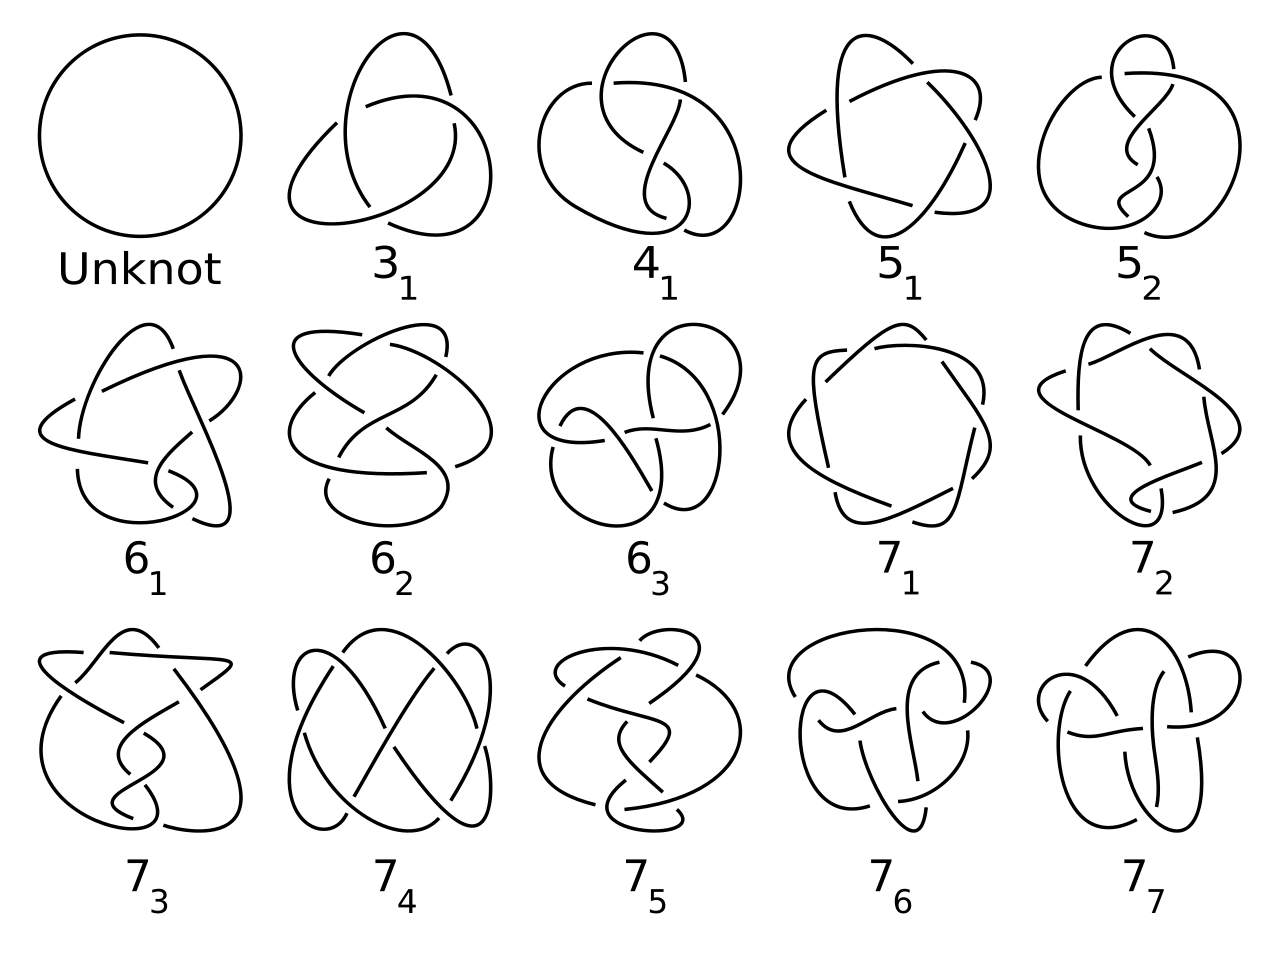
\includegraphics[scale=0.25]{4/knoty.png}
\caption{Niewęzeł i węzły pierwsze o mniej niż 8 skrzyżowaniach.}
\end{figure}